\documentclass [11pt,twoside]{article}
\usepackage[utf8]{inputenc}
\usepackage[T1]{fontenc}

%Page margins, header and footer positions
\usepackage{geometry}
 \geometry{
 a4paper,
 total={210mm,297mm},
 left=25mm,
 right=25mm,
 top=30mm,
 bottom=25mm,
 headsep=7mm}

\interfootnotelinepenalty=10000

%To display filling dots in the TOC for all entries
\usepackage[titles]{tocloft}
\renewcommand{\cftsecleader}{\cftdotfill{\cftdotsep}}

%Define new header and footer style
\usepackage{fancyhdr}

\pagestyle{fancy}
\fancyhf{}
\lhead{\color{Gray}{\small{Model Checking of Battery-Powered Railway Lines project by Lorenzo Iovine, Nicola Landini, Francesco Leone}}}
\lfoot{\textcolor{Gray}{\small{Copyright © 2022, Lorenzo Iovine, Nicola Landini, Francesco Leone – All rights reserved}}}
\rfoot{\textcolor{Gray}{\thepage}}
\renewcommand{\headrulewidth}{0pt}

%PACKAGES
\usepackage{wasysym}
\usepackage{pifont}

\newcommand{\supported}{\ding{52}\xspace}
\newcommand{\unsupported}{\ding{55}\xspace}
\newcommand{\partsupported}{\textcolor{black!40}{\ding{52}}\xspace}
\newcommand{\lowsupported}{\textcolor{black!20}{\ding{52}}\xspace}
\newcommand{\unknowsupported}{\textbf{?}\xspace}

%Font: Times
\usepackage{times}
%Change monospaced font
\renewcommand{\ttdefault}{lmtt}

%tables
\usepackage{tabu}
\usepackage{tabularx}
\usepackage{ltablex}
\usepackage{longtable}
\usepackage{float} % To allow the use of H modifier in long tables

%landscape mode
\usepackage{pdflscape}
\usepackage{rotating}
\usepackage{caption}

%make landscape mode be sensitive to even and odd pages
%start
\def\myrotate{\ifodd\c@page\else-\fi 90}
\makeatletter
\global\let\orig@begin@landscape=\landscape%
\global\let\orig@end@landscape=\endlandscape%
\gdef\@true{1}
\gdef\@false{0}
\gdef\landscape{%
    \global\let\within@landscape=\@true%
    \orig@begin@landscape%
}%
\gdef\endlandscape{%
    \orig@end@landscape%
    \global\let\within@landscape=\@false%
}%
\@ifpackageloaded{pdflscape}{%
    \gdef\pdf@landscape@rotate{\PLS@Rotate}%
}{
    \gdef\pdf@landscape@rotate#1{}%
}
\let\latex@outputpage\@outputpage
\def\@outputpage{
    \ifx\within@landscape\@true%
        \if@twoside%
            \ifodd\c@page%
                \gdef\LS@rot{\setbox\@outputbox\vbox{%
                    \pdf@landscape@rotate{-90}%
                    \hbox{\rotatebox{90}{\hbox{\rotatebox{180}{\box\@outputbox}}}}}%
                }%
            \else%
                \gdef\LS@rot{\setbox\@outputbox\vbox{%
                    \pdf@landscape@rotate{+90}%
                    \hbox{\rotatebox{90}{\hbox{\rotatebox{0}{\box\@outputbox}}}}}%
                }%
            \fi%
        \else%
            \gdef\LS@rot{\setbox\@outputbox\vbox{%
                \pdf@landscape@rotate{+90}%
                \hbox{\rotatebox{90}{\hbox{\rotatebox{0}{\box\@outputbox}}}}}%
            }%
        \fi%
    \fi%
    \latex@outputpage%
}
\makeatother
%end

%graphics
\usepackage{graphicx}
\usepackage[dvipsnames, table]{xcolor}
%If you upload images from PC, you need to insert code for the path here (different for Windows and Unix OS)

%References
%\usepackage{xpatch}
%\usepackage[backend=biber, style=numeric, citestyle=numeric, sorting=none]{biblatex}
%\addbibresource{main.bib}

%Other
\usepackage{ifthen}
%! suppress = MultipleIncludes
\usepackage{xspace}
\usepackage{enumitem}
\usepackage{amssymb}
\usepackage[pdftex, colorlinks]{hyperref}
\newcommand{\comment}[1]{{\color{Red}$\blacktriangleright$ Comment: #1 $\blacktriangleleft$}}


% Some utilities\ldots
\usepackage{soul}
\usepackage{tikz}

\usetikzlibrary{calc}
\usetikzlibrary{decorations.pathmorphing}


\makeatletter

\newcommand{\defhighlighter}[3][]{%
  \tikzset{every highlighter/.style={color=#2, fill opacity=#3, #1}}%
}

\defhighlighter{yellow}{.5}

\newcommand{\highlight@DoHighlight}{
  \fill [ decoration = {random steps, amplitude=1pt, segment length=15pt}
        , outer sep = -15pt, inner sep = 0pt, decorate
       , every highlighter, this highlighter ]
        ($(begin highlight)+(0,8pt)$) rectangle ($(end highlight)+(0,-3pt)$) ;
}

\newcommand{\highlight@BeginHighlight}{
  \coordinate (begin highlight) at (0,0) ;
}

\newcommand{\highlight@EndHighlight}{
  \coordinate (end highlight) at (0,0) ;
}

\newdimen\highlight@previous
\newdimen\highlight@current

\DeclareRobustCommand*\highlight[1][]{%
  \tikzset{this highlighter/.style={#1}}%
  \SOUL@setup
  %
  \def\SOUL@preamble{%
    \begin{tikzpicture}[overlay, remember picture]
      \highlight@BeginHighlight
      \highlight@EndHighlight
    \end{tikzpicture}%
  }%
  %
  \def\SOUL@postamble{%
    \begin{tikzpicture}[overlay, remember picture]
      \highlight@EndHighlight
      \highlight@DoHighlight
    \end{tikzpicture}%
  }%
  %
  \def\SOUL@everyhyphen{%
    \discretionary{%
      \SOUL@setkern\SOUL@hyphkern
      \SOUL@sethyphenchar
      \tikz[overlay, remember picture] \highlight@EndHighlight ;%
    }{%
    }{%
      \SOUL@setkern\SOUL@charkern
    }%
  }%
  %
  \def\SOUL@everyexhyphen##1{%
    \SOUL@setkern\SOUL@hyphkern
    \hbox{##1}%
    \discretionary{%
      \tikz[overlay, remember picture] \highlight@EndHighlight ;%
    }{%
    }{%
      \SOUL@setkern\SOUL@charkern
    }%
  }%
  %
  \def\SOUL@everysyllable{%
    \begin{tikzpicture}[overlay, remember picture]
      \path let \p0 = (begin highlight), \p1 = (0,0) in \pgfextra
        \global\highlight@previous=\y0
        \global\highlight@current =\y1
      \endpgfextra (0,0) ;
      \ifdim\highlight@current < \highlight@previous
        \highlight@DoHighlight
        \highlight@BeginHighlight
      \fi
    \end{tikzpicture}%
    \the\SOUL@syllable
    \tikz[overlay, remember picture] \highlight@EndHighlight ;%
  }%
  \SOUL@
}

\makeatother

% Common abbrev. are set as commands to ensure proper spacing after the dot
\RequirePackage{xspace}
\newcommand{\ie}{i.e.\@\xspace}
\newcommand{\aka}{a.k.a.\@\xspace}
\newcommand{\Ie}{I.e.\@\xspace}
\newcommand{\cf}{cf.\@\xspace}
\newcommand{\Cf}{Cf.\@\xspace}
\newcommand{\eg}{e.g.\@\xspace}
\newcommand{\Eg}{E.g.\@\xspace}
\newcommand{\etal}{et al.\@\xspace}
\newcommand{\etc}{etc.\@\xspace}
\newcommand{\wrt}{w.r.t.\@\xspace}
\newcommand{\Wrt}{W.r.t.\@\xspace}



\date{}

\usepackage{listings}

\begin{document}

%TITLE PAGE

%LOGO

{\begin{titlepage}
     \begin{center}
         
\includegraphics[width=0.4\textwidth]{images/PolimiLogo.png}

         \vspace{0.2cm}

         \Large Computer Science and Engineering

         \vspace{0.9cm}

         \Huge \textbf{Model Checking of Battery-Powered Railway Lines}

         \vspace{0.7cm}
         \huge Formal Method for Concurrent and Real Time Systems Project

         \vspace{1.5cm}
         \Large Academic year 2021 - 2022\\
         \vspace{1cm}
         24 June 2022\\Version 1.0
         \vspace{3cm}

         \large
         \begin{minipage}{.1\textwidth}
             \null
         \end{minipage}%
         \begin{minipage}{.4\textwidth}
             \textit{Authors}:\\
             Lorenzo IOVINE\\
             Nicola LANDINI\\
             Francesco LEONE
         \end{minipage}%
         \begin{minipage}{.4\textwidth}
             \raggedleft
             \textit{Istruttors}:\\
             Prof. Pierluigi SAN PIETRO\\
             Dr. Livia LESTINGI\\
             \phantom{placeholder}
         \end{minipage}%
         \begin{minipage}{.1\textwidth}
             \null
         \end{minipage}


     \end{center}
\end{titlepage}}~\\

%TITLE

%Define deliverable specific info
%Replace cell contents where needed
\begin{table}[h!]
    \begin{tabu} to \textwidth { X[0.3,r,p] X[0.7,l,p] }
    \hline

    \textbf{Deliverable:} & Formal Method for Concurrent and Real Time Systems project\\
    \textbf{Title:} & Model Checking of Battery-Powered Railway Lines \\
    \textbf{Authors:} & Lorenzo Iovine, Nicola Landini, Francesco Leone\\
    \textbf{Version:} & 1.0 \\
    \textbf{Date:} & 24-June-2022 \\
    \textbf{Copyright:} & Copyright © 2022, Lorenzo Iovine, Nicola Landini, Francesco Leone – All rights reserved \\
    \hline
    \end{tabu}
\end{table}




\setcounter{page}{2}


%------------------------------------------------------------------------------------------------------------------------------------------------
\newpage
\addcontentsline{toc}{section}{Table of Contents}
\tableofcontents
\newpage
\addcontentsline{toc}{section}{List of Figures}
\listoffigures

%------------------------------------------------------------------------------------------------------------------------------------------------
\clearpage
{\color{Blue}{\section{Design}}}
\label{sect:design}
\subsection{Purpose}
The fight to reduce greenhouse gas emissions is bringing together researchers and manufacturers from all over the world.
In particular, rechargeable batteries as a source of power in place of fossil fuels are already widespread in cars and
making their way into the rail transport sector. Battery-powered trains are already operative in several countries like
Japan, Austria, and Britain. Italy is also planning on producing and deploying fully-electric trains starting mid-2022,
thanks to a deal with Hitachi Rail.\\
\\ Like any electric vehicle, trains can cover a limited distance running only on battery power before needing to recharge.
In this project, we will model a railway line in which electric trains can recharge in a station. Nevertheless,
trains must still reach the following station on time; in case of excessive delay, the company is obliged to issue
monetary compensation to the passengers.\\
\\ Precisely, given a set of simplifying assumptions, we will model the main actors of the system as a network of \textbf{Timed Automata (TA)}
whose behavior depends on specific key parameters.


\bigskip
\subsection{High Level Model Description}
We created two different configurations for the railway model. Both of them include 4 trains and 3 stations.\\
The first one represents the main configuration of the system and verifies all the properties. The railway model is set as follows:
\\
\begin{figure}[H]
    \centering
    
\includegraphics[scale=0.4]{images/poweredRailway.png}
\end{figure}
\bigskip

The second configuration doesn't verify the mandatory properties of the project and it is set as follows:
\\
\begin{figure}[H]
    \centering
    
\includegraphics[scale=0.4]{images/poweredRailwaySimple.png}
\end{figure}
\bigskip

\subsection{Initializations}
The stations have the following initial configurations:
\begin{itemize}
    \item \textbf{Station 0: } 2 tracks, 1 available
    \item \textbf{Station 1: } 3 tracks, 2 available
    \item \textbf{Station 2: } 2 tracks, 0 available
\end{itemize}
\newpage

The trains that we designed have constant speed set to 120 km/h. They are initialized as follows:
\begin{itemize}
    \item \textbf{Train 0 - charge 100: } starts from station 0 with station 2 as destination
    \item \textbf{Train 1 - charge 100: } starts from station 1 with station 2 as destination
    \item \textbf{Train 2 - charge 100: } starts from station 2 with station 0 as destination
    \item \textbf{Train 3 - charge 100: } starts from station 2 with station 0 as destination
\end{itemize}
\bigskip

\subsection{Design assumptions}
In order to efficiently describe the model, we decided to make the following assumptions:
\begin{itemize}
    \item Every station has less tracks than the total number of trains.
    \item A clock unit is equal to a minute.
    \item For each train the destination is the last station, except for the one that start from the last one who has
    as destination the first station.
    \item The lower bound to allow passengers to get on and off the train is of 4 clock unit.
    \item We set a charging multiplier and two different discharging multiplier, one for the waiting and one for the travel.
\end{itemize}

\bigskip

\subsection{Design Choices}
\begin{itemize}
    \item We decided not to design the railway with a dedicated template. That's because the railway's most important features
    are implicitly designed and verified, without creating additional variables.
    \item In order to save time when checking properties we avoid redundant clocks for operations that are not issued in parallel.
    \item Our \emph{Recharge Policy} is based on a control made in function \textit{chargingTime} in the \textit{Train Template},
    that allows to recharge the train at least for the lower bound (described before). In case the train needs more time to 
    recharge in order to get to the next station, the time spent in the station is the mean value between the lower bound
    and the upper bound (calculated as follows: $MaximumDelay-\frac{DistanceToNextStation}{trainSpeed}$) in order not 
    to overcome the maximum delay. We thought that this is a good compromise between charging the train and have some delay 
    in reaching the next station.
    \item In order to model the station, the distances and the maximum delays between stations we used two matrices. It is enough 
    to change the number of trains/stations, initialize them and update the matrices, and the system will "adapt" to the 
    new configuration.
    \item All the variables that could be declared as constant, are declared as constant, in order to save time when checking properties.
\end{itemize}



%------------------------------------------------------------------------------------------------------------------------------------------------
\clearpage
{\color{Blue}{\section{UPPAAL Model}}}
\label{sect:uppaal}
\subsection{Global Declarations}
\subsubsection{System Parameters}

\begin{table} [H]
    \begin{tabu} to \textwidth {|X|X[2]|}
        \hline
        \textbf{Parameter}              & \textbf{Description} \\  \hline
        nStations                       & Number of stations in the system \\  \hline
        nTrains                         & Number of trains in the system \\    \hline
        chargingSpeed                   & A multiplier for the battery charging speed \\    \hline
        journeyDischargeMultiplier      & A multiplier for the battery discharge during the journey \\  \hline
        waitingDischargeMultiplier      & A multiplier for the battery discharge during the waiting \\  \hline
        MIN\_TIME\_PER\_STATION         & Lower bound to allow passengers to get on and off the train \\    \hline
        trainSpeed                      & Trains' speed \\   \hline
        stationNumOfTracks              & Array with the number of tracks of each station \\   \hline
        railLine\_distance              & Matrix containing the distance between stations \\    \hline
        railLine\_delay                 & Matrix containing the maximum delay between stations \\   \hline
    \end{tabu}
\end{table}
\bigskip

\subsubsection{System Variables}
\begin{table} [H]
    \begin{tabu} to \textwidth {|X|X[2]|}
    \hline
    \textbf{Variable}          & \textbf{Description} \\  \hline
    trainStation                & Array with the current station of each train \\  \hline
    trainDestination            & Array with the destination of each train \\   \hline
    nextStop                    & Array with the next station of each train \\  \hline
    stationFreeTracks           & Array with the current number of free tracks of each station \\   \hline
    chargeOfTrain               & Array with the current charge of each train battery \\    \hline
    \end{tabu}
\end{table}
\bigskip

\subsubsection{System Channels}
\begin{table} [H]
    \begin{tabu} to \textwidth {|X|X[2]|}
    \hline
    \textbf{Channel}          & \textbf{Description} \\  \hline
    exitTrain                   & Channels through which a train inform its current station that it is leaving \\  \hline
    full                        & Channels through which a station communicate to an incoming train that it has no available tracks\\  \hline
    allowedIn                   & Channels through which a station grant the access to a train that is waiting \\ \hline
    arrived                     & Channels through which a train inform its next station that it is arrived\\ \hline
    \end{tabu}
\end{table}

\newpage

\subsection{Templates}
\subsubsection{Station}
\begin{figure}[H]
    \centering
    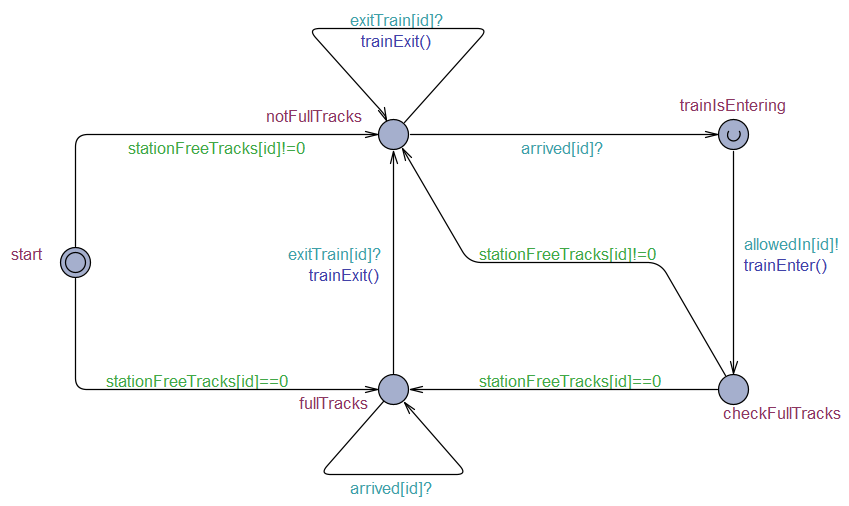
\includegraphics[scale=0.9]{images/stationTemplate.png}
\end{figure}

\begin{itemize}
    \item \textbf{start: }this is the initial state of the Station Template. In case the number of available
            tracks is equal to zero the next state is notFullTracks, otherwise the next state is \emph{fullTracks}.
    \item \textbf{notFullTracks: }when this state receives a message on the \emph{exitTrain} channel, it updates his 
            \emph{stationFreeTracks} variable and the current state doesn't change. Upon receiving a message on the 
            \emph{arrived} channel the current state moves to \emph{checkFreeTracks} state.
    \item \textbf{fullTracks: }when this state receives a message on the \emph{arrived} channel the current state doesn't change. 
            Instead, if this state receives a message on the \emph{exitTrain} channel, it updates his \emph{stationFreeTracks} 
            variable and the current state moves to \emph{notFullTracks} state.
    \item \textbf{trainIsEntering: }this is an urgent state created to describe when a train is joining the station.
    \item \textbf{checkFullTracks: }this state is reached immediately after the update of the \emph{stationFreeTracks} variable
            and checks if the station has available tracks. In this case the current state becomes \emph{notFullTracks},
            otherwise it becomes \emph{fullTracks}.
\end{itemize}
\newpage

\subsubsection{Train}
\begin{figure}[H]
    \centering
    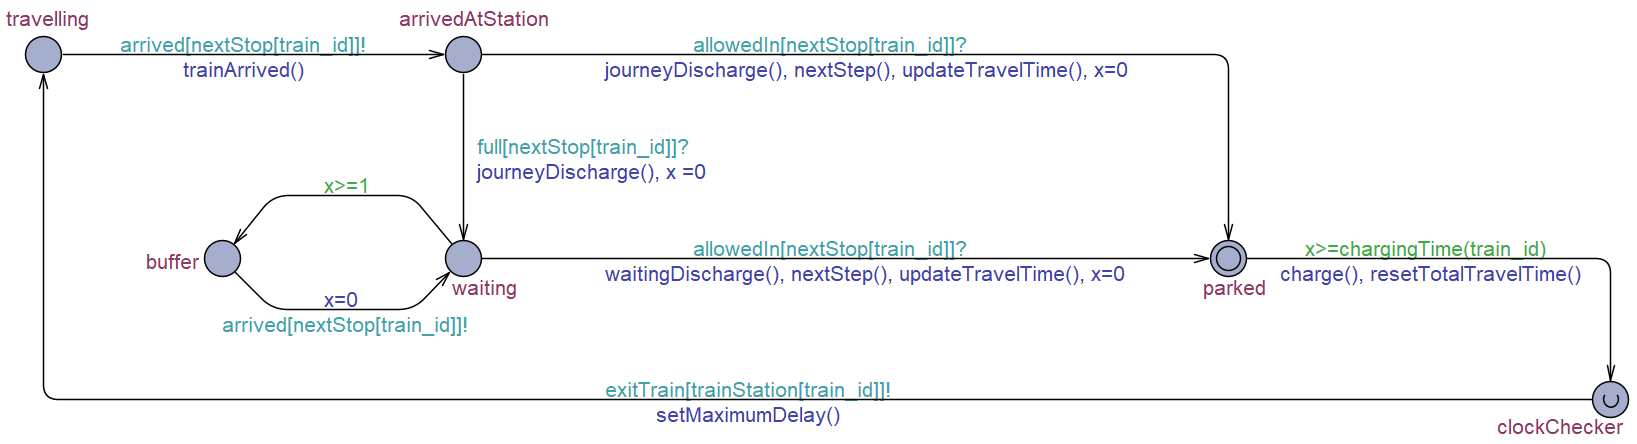
\includegraphics[scale=0.56]{images/trainTemplate.png}
\end{figure}

\begin{itemize}
    \item \textbf{parked: }this is the initial state of the Train Template. It represents the situation in which the train is
            stopped in a station. The current state changes only if the clock is greater or equal to the needed charging time.
            Before the current state changes in \emph{clockChecker} we compute the \emph{charge} method that increases the
            train battery linearly with the time spent in the station.
    \item \textbf{clockChecker: }this is an urgent state created to send a message on \emph{exitTrain} channel and to set
            the maximum delay to reach the next station.
    \item \textbf{travelling: }this state represents the situation in which the train left the previous station and heads to
            the next one. Before reaching the next station, we send a message on \emph{arrived} channel to inform the station
            of the arrival and update train's current station.
    \item \textbf{arrivedAtStation: }this state checks if the train has to wait before entering or if it is allowed to join 
            the station. In the first case the current state becomes \emph{waiting} after receiving a message on \emph{full}
            channel, otherwise the system comes back to the initial state after receiving a message on \emph{allowedIn} channel.
            Before reaching one of the next state we compute the \textit{journeyDischarge} method that decreases
            the train battery linearly with the travel time.
    \item \textbf{waiting: }this is the state in which the train waits until the station, throw \emph{allowedIn} channel,
            allows him to join. Before entering the station we compute the \textit{waitingDischarge} method that decreases
            the train battery linearly with the waiting time.
    \item \textbf{waiting-buffer: }this is a snippet of Train Template that describes the loop in which the train is while
            waiting to be allowed to join the next station. In this loop we send a message through \emph{arrived} channel
            to the station every clock time unit.
            \begin{figure}[H]
                \centering
                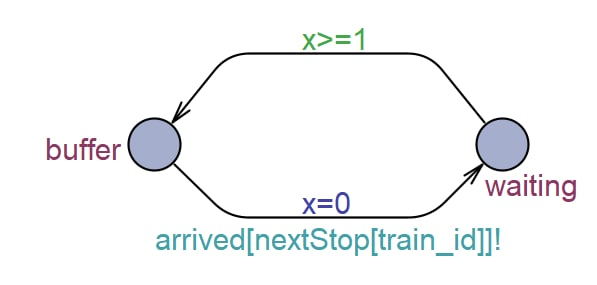
\includegraphics[scale=0.56]{images/bufferSnippet.png}
            \end{figure}
\end{itemize}

\newpage

\begin{table} [H]
    \begin{tabu} to \textwidth {|X|X[3.5]|}
    \hline
    \textbf{Train local variables}              & \textbf{Description} \\  \hline
    x                       & This is the clock used to temporalize the system \\  \hline
    totalTravelTime         & An int that represents the overall time to reach the next station \\    \hline
    parkedTime              & An int that represents the time spent in a station \\    \hline
    travelTime              & An int that represents the time spent in the journey \\  \hline
    waitingTime             & An int that represents the time wasted until the station authorizes the access \\  \hline
    actualMaximumDelay      & An int used to save the maximum delay allowed to reach the next station \\    \hline
    \end{tabu}
\end{table}

\newpage



%------------------------------------------------------------------------------------------------------------------------------------------------
\clearpage
{\color{Blue}{\section{Analysis and Results}}}
\label{sect:result}
\subsection{Property Verification}
\subsubsection{Mandatory Properties}
In this section we will describe the analyzed properties. The first two properties analyzed are the compulsory ones:
\begin{itemize}
    \item $\forall  \square(chargeOfTrain[Train\_id] > 0) $
    \item $\forall \square(train.totalTravelTime <= train.actualMaximumDelay) $
\end{itemize}

We have created two configuration of the system: in the first one the two properties are satisfied, in the second one not.
The difference between the two configuration is the max delay allowed.

\paragraph{Configuration1} In this configuration the properties are satisfied \begin{itemize}
    \item Max Delay Station 1-2 : 50
    \item Max Delay Station 2-3 : 60
\end{itemize}



\paragraph{Configuration2}
In this configuration the properties are not satisfied \begin{itemize}
    \item Max Delay Station 1-2 : 25
    \item Max Delay Station 2-3 : 30
\end{itemize} The two properties could be satisfied even in this configuration if we increase the \textit{chargingMultiplier}


\subsubsection{Additional Properties}
We have written two additional properties, the first one to check that the number of free Tracks in a station is always greater or equal to 0,
the second one to check that every train eventually reaches its destination.
\begin{itemize}
    \item $\forall  \square(stationFreeTracks[station\_id] >=  0) $
    \item $\forall  \lozenge(trainStation[Train\_id] = trainDestination[Train\_id]) $
\end{itemize}
Both properties are satisfied in both configuration of the system.


%------------------------------------------------------------------------------------------------------------------------------------------------
\clearpage
{\color{Blue}{\section{Conclusion}}}
\label{sect:conclusion}
In this report we presented an analysis of the problem of the Model Checking of Battery Powered Railway Lines.
The aim was to check a realistic configuration in order to understand the validity of the model.\\
From the results showed, we succeeded in finding a configuration where all the properties to be checked are satisfied.
We also tried to increase verification performances by reducing the state space, in order to decrease processing time.
The main characteristic that emerged are the recharge policies. The real bottleneck of the system is the fact that
there are stations with a number of tracks lower than trains in the system. It is important to find a consistent recharge
policy in order to efficiently describe the behavior of the system without letting the parameters to be inconsistent.\\
This project allowed us to improve our team working and knowledge about the subjects of the course.


%------------------------------------------------------------------------------------------------------------------------------------------------



\end{document}
